\documentclass[utf8,english]{gradu3}
% If you are writing a Bachelor's Thesis, use the following instead:
%\documentclass[utf8,bachelor,english]{gradu3}

\usepackage{graphicx} % for including pictures

\usepackage{amsmath} % useful for math (optional)

\usepackage{booktabs} % good for beautiful tables

% NOTE: This must be the last \usepackage in the whole document!
\usepackage[bookmarksopen,bookmarksnumbered,linktocpage]{hyperref}

\graphicspath{ {img/} }
\addbibresource{bibliography.bib} % The file name of your bibliography database

\begin{document}

\title{Migrating a web application to serverless architecture}
\translatedtitle{Web-sovelluksen siirtäminen serverless-arkkitehtuuriin}
\studyline{Master's Thesis in Information Technology}
\avainsanat{%
  serverless,
  FaaS,
  arkkitehtuuri,
  pilvilaskenta,
  web-sovellukset}
\keywords{
  serverless,
  FaaS,
  architecture,
  cloud computing,
  web applications}
\tiivistelma{%
  Tämä kirjoitelma on esimerkki siitä, kuinka
  {gradu3}-tutkielmapohjaa käytetään.  Se sisältää myös
  käyttöohjeet ja tutkielman rakennetta koskevia ohjeita.

  Tutkielman tiivistelmä on tyypillisesti lyhyt esitys, jossa
  kerrotaan tutkielman taustoista, tavoitteesta, tutkimusmenetelmistä,
  saavutetuista tuloksista, tulosten tulkinnasta ja johtopäätöksistä.
  Tiivistelmän tulee olla niin lyhyt, että se, englanninkielinen
  abstrakti ja muut metatiedot mahtuvat kaikki samalle sivulle.

  Sen tulee kertoa täsmälleen samat asiat kuin englannikielinen
  abstrakti.
}
\abstract{%
  This document is a sample {gradu3} thesis document class
  document.  It also functions as a user manual and supplies
  guidelines for structuring a thesis document.

  The abstact is typically short and discusses the background, the
  aims, the research methods, the obtained results, the interpretation
  of the results and the conculsions of the thesis.  It should be so
  short that it, the Finnish translation, and all other meta
  information fit on the same page.

  The Finnish tiivistelmä of a thesis should usually say exactly the same
  things as the abstract.
}

\author{Aleksi Pekkala}
\contactinformation{\texttt{alvianpe@student.jyu.fi}}
% use a separate \author command for each author, if there is more than one
\supervisor{Oleksiy Khriyenko}
% use a separate \supervisor command for each supervisor, if there
% is more than one

\maketitle

% \begin{thetermlist}
% \item[FaaS] Function as a Service.
% % \item[\LaTeX] A system, built on top of \TeX\
% %   \parencite{knuth86:_texbook}, for typesetting structured
% %   documents \parencite[see][]{lamport94:_latex}.  Its current version
% %   is \LaTeXe.
% \end{thetermlist}

\mainmatter

\chapter{Introduction}

Cloud computing has in the past decade emerged as a veritable backbone of modern economy, driving innovation both in industry and academia as well as enabling scalable global enterprise applications. Just as the adoption of cloud computing continues to increase, the technologies in which the paradigm is based have continued to progress. Recently the development of novel virtualization techniques has lead to the introduction of \textit{serverless computing}, an architectural pattern based on ephemeral cloud resources that scale up and down automatically and are billed for actual usage at a millisecond granularity. The main drivers behind serverless computing are to both reduce operational costs by more efficient cloud resource utilization and to improve developer productivity by shifting provisioning, load balancing and other infrastructure concerns to the platform. \parencite{buyya2017manifesto}

As an appealing economic proposition, serverless computing has attracted significant interest in the industry. This is illustrated for example by its appearance in the 2017 Gartner Hype Technologies Report \parencite{walker17gartnerHype}. By now most of the prominent cloud service providers have introduced their own serverless platforms, promising capabilities that make writing scalable web services easier and cheaper \parencite[e.g.][]{awslambda0218, google18cloudFunctions, ibm18cloudFunctions, microsoft18azureFunctions}. A number of high-profile use cases have also been presented in the literature \parencite{cncf18serverlessWG}. \textcite{baldini17currentTrends} however note a lack of corresponding degree of interest in academia despite a wide variety of technologically challenging and intellectually deep problems in the space.

One of the open problems identified in literature concerns the discovery of serverless design patterns: how do we compose the granular building blocks of serverless into larger systems? \parencite{baldini17currentTrends} \textcite{varghese18next} contend that one challenge hindering the widespread adoption of serverless will be the radical shift in the properties that a programmer will need to focus on, from latency, scalability and elasticity to those relating to the modularity of an application. Considering this and the paradigm's unique characteristics and limitations, it's unclear to what extent our current patterns apply and what kind of new patterns are best suited to optimize for the features of serverless computing. The object of this thesis is to fill the gap by re-evaluating existing design patterns in the serverless context and proposing new ones through an exploratory migration process.

\section{Research problem}

The research problem addressed by this thesis distills down to 4 different questions:
\begin{enumerate}
  \item Why should a web application be migrated to serverless?
  \item What kind of patterns are there for building serverless web application backends?
  \item Do the existing patterns have gaps or missing parts, and if so, can we come up with improvements or alternative solutions?
  \item How does migrating a web application to serverless affect its quality?
\end{enumerate}

The first two questions are addressed in the theoretical part of the thesis. Question 1 concerns the motivation behind the thesis and introduces serverless migration as an important and relevant business problem. Question 2 is answered by surveying existing literature for serverless patterns as well as other, more general patterns thought suitable for the target class of applications.

The latter questions form the constructive part of the thesis. Question 3 concerns the application and evaluation of surveyed patterns. The surveyed design patterns are used to implement a subset of an existing traditional web application in the serverless architecture. In case the patterns prove unsuitable for any given problem, alternative solutions or extensions are proposed. The last question consists of comparing the migrated portions of the app to the original version and evaluating whether the posited benefits of serverless architecture are in fact realized.

\section{Outline}

The thesis is structured as follows: the second chapter serves as an introduction to the concept of serverless computing. The chapter describes the main benefits and drawbacks of the platform, as well as touching upon its internal mechanisms and briefly comparing the main service providers. Extra emphasis is placed on how the platform's limitations should be taken into account when designing web application backends.

The third chapter consists of a survey into existing serverless design patterns and recommendations. Applicability of other cloud computing, distributed computing and enterprise integration patterns is also evaluated.

The fourth chapter describes the process of migrating an existing web application to serverless architecture. The patterns discovered in the previous chapter are utilized to implemented various typical web application features on a serverless platform. In cases where existing patterns prove insufficient or unsuitable as per the target application's characteristics, modifications or new patterns are proposed.

The outcome of the migration process is evaluated in the fifth chapter. The potential benefits and drawbacks of the serverless platform outlined in chapter 2 are used to reflect on the final artifact. The chapter includes approximations on measurable attributes such as hosting costs and performance as well as discussion on the more subjective attributes like maintainability and testability. The overall ease of development -- or developer experience -- is also addressed since it is one of the commonly reported pain points of serverless computing \parencite{van2017spec}.

The final chapter of the thesis aims to draw conclusions on the migration process and the resulting artifacts. The chapter contains a summary of the research outcomes and ends with recommendations for further research topics.


\chapter{Serverless computing} \label{cha:serverless}

This chapter serves as an introduction to serverless computing. Defining serverless computing succinctly can be difficult because of the relative immaturity of the field. The NIST definitions of cloud computing have yet to catch up with the technology \parencite{nist11definitions}, and an effort to formalize and standardize serverless computing by the industry-headed Cloud Native Computing Foundation is still underway \parencite{cncf18serverlessWG}. As a result the boundaries between serverless and other cloud computing terms are still somewhat blurred, and the terms seem to carry slightly different meanings depending on the author or context. To complicate matters further, serverless computing has come to appear in two different but overlapping forms. A multilayered approach is therefore in order.

We approach the formidable task of defining serverless by first taking a brief look at the history and motivations behind utility computing. After that we'll introduce the basic tenets of serverless computing, distinguish between its two main approaches and see how it positions itself relative to other cloud service models. This is followed by a more technical look at the most recent serverless model, as well as its major providers, use cases, security issues and economic implications. The chapter closes with notes on the drawbacks and limitations of serverless, particularly from the point of view of web application backends. This thesis' definition of serverless leans heavily on the CNCF Serverless Working Group's whitepaper \parencite{cncf18serverlessWG}, the seminal introduction to the topic by \textcite{robert2016serverlessarchitectures} as well as a number of recent survey articles \parencite[e.g.][]{baldini17currentTrends,van2017spec,fox17}

As a sidenote, although the earliest uses of term 'serverless' can be traced back to peer-to-peer and client-only solutions \parencite{fox17}, we're dismissing these references since the name has evolved into a completely different meaning in the current cloud computing context. As per \textcite{robert2016serverlessarchitectures}, first usages of the term referring to elastic cloud computing seem to have appeared in around 2012.

% TODO: How does serverless relate to concepts such as FaaS, BaaS/MBaaS like Auth0 and Firebase, SOA, microservices, event-driven, virtualization, containers, cloud-native, ...? Cloud-ready/cloud-native as defined by \textcite{pozdniakova17cloudready}.

\section{Background} \label{sec:background}

Utility computing refers to a model where computing resources, such as computation and storage, are commoditized and delivered as metered services in a similarly to physical public utilities such as water, electricity and telephony. Utilities are readily available to consumers at any time whenever required and billed per actual usage. In computing, this has come to mean on-demand access to highly scalable subscribtion-based IT resources. The availability of computing as an utility enables organizations to avoid investing heavily on building and maintaining complex IT infrastructure. \parencite{buyya09cloud}

This vision of utility computing can be traced all the way back to 1961, with the computing pioneer John McCarthy predicting that "computation may someday be organized as a public utility" \parencite{foster08cloudGrid}. Likewise in 1969 Leonard Kleinrock, one of the chieft scientists in the ARPANET project, is quoted as saying, "as of now, computer networks are still in their infancy, but as they grow up and become sophisticated, we will probably see the spread of ‘computer utilities’ which, like present electric and telephone utilities, will service individual homes and offices across the country" \parencite{kleinrock03internet}. The creation of the Internet first facilitated weaving computer resources together into large-scale distributed systems. Onset by this discovery, multiple computing paradigms have been proposed and adopted over the years to take on the role of a ubiquitous computing utility, including cluster, grid, peer-to-peer (P2P) and services computing \parencite{buyya09cloud}. The latest paradigm, cloud computing, has in the past decade revolutionized the computer science horizon and got us closer to computing as an utility than ever. \parencite{buyya2017manifesto}.

\textcite{sareen13cloudTypes} succinctly defines the cloud as a pool of virtualized computer resources. \textcite{foster08cloudGrid} present a more thorough definition of cloud computing as "a large-scale distributed computing paradigm that is driven by economies of scale, in which a pool of abstracted, virtualized, dynamically-scalable, managed computing power, storage, platforms, and services are delivered on demand to external customers over the Internet". Cloud computing builds on the earlier paradigm of grid computing, and relies on grid computing as its backbone and infrastructure. Compared to infrastructure-based grid computing, cloud computing focuses on more abstract resources and services. \textcite{buyya2017manifesto} also note that cloud computing differs from grid computing in that it
promises virtually unlimited computational resources on demand.

% expound on IaaS/PaaS/SaaS here?

The first cloud providers were born out of huge corporations offering their surplus computing resources as a service in order to offset expenses and improve utilization rates. Having set up global infrastructure to handle peak demand, a large part of the resources were left under-utilized at times of average demand. The providers are able to offer these surplus resources at attractive prices due to the large scale of their operations, benefiting from economies of scale. To address consumers' concerns about outages and other risks, cloud providers guarantee a certain level of service delivery through Service Level Agreements (SLA) that are negotiated between providers and consumers. \parencite{youseff08cloudOntology}

The key technology that enables cloud providers to transparently handle consumers' requests without impairing their own processing needs is \textit{virtualization}. Virtualization is one of the main components behind cloud computing and one of the factors setting it apart from grid computing. \textcite{sareen13cloudTypes} defines virtualization as using computer resources to imitate other computer resources or whole computers. This enables the abstraction of the underlying physical resources as a set of multiple logical virtual machines (VM). Virtualization has three characteristics that make it ideal for cloud computing: 1) \textit{partitioning} supports running many applications and operating systems in a single physical system; 2) \textit{isolation} ensures boundaries between the host physical system and virtual containers; 3) \textit{encapsulation} enables packaging virtual machines as complete entities to prevent applications from interfering with each other.
% foster08 has more on virtualization

Virtual machines provide strong security guarantees by isolation, i.e. allocating each VM its own set of resources with minimal sharing between the host system. Minimal sharing however translates into high memory and storage requirements as each virtual machine requires a full OS image in addition to the actual application files. A virtual machine also has to go through the standard OS boot process on startup, resulting in launching times measured in minutes. Rapid innovation in the cloud market and virtualization technologies has recently lead to an alternative, more lightweight \textit{container}-based solution. Container applications share a kernel with the host, resulting in significantly smaller deployments and fast launching times ranging from less than a second to a few seconds. Due to resource sharing a single host is capable of hosting hundreds of containers simultaneously. Differences in resource sharing between VM- and container-based deployment is illustrated in figure \ref{fig:vmVsContainer}. As a downside containers lack the VM's strong isolation guarantee and the ability to run a different OS per deployment. On the other hand, containers provide isolation via namespaces, so processes inside containers are still isolated from each other as well as the host. \textit{Containerization} has emerged as a common practice of packaging applications and related dependencies into standardized container images to ease development efficiency and interoperability. \parencite{pahl15containerization}
% mention CaaS, kubernetes etc
% he container technology due to its small footprint and fast deployment is crucial in serverless

\begin{figure}[h]
  \centering
  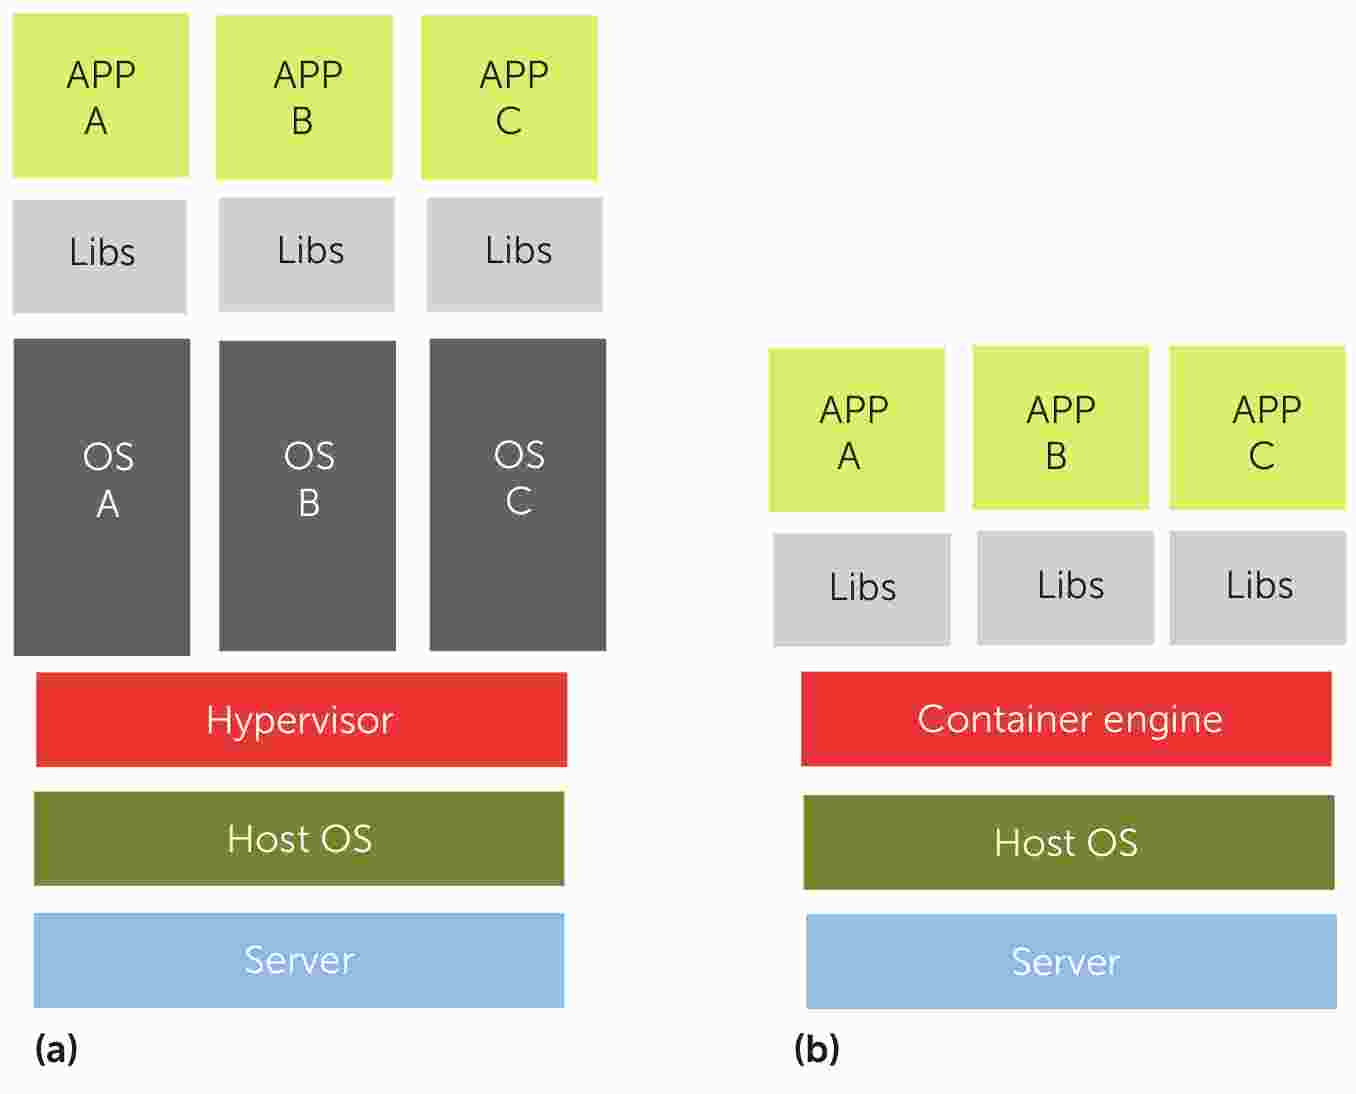
\includegraphics[width=\textwidth]{bernstein14-vm-vs-container.jpg}
  \caption{Comparison of a) virtual machine- and b) container-based deployments \parencite{bernstein14containers}}
  \label{fig:vmVsContainer}
\end{figure}

Cloud computing is by now a well-established paradigm that enables organizations to flexibly deploy a wide variety of software systems over a pool of externally managed computing resources. Both major IT companies and startups see migrating on-premise legacy systems to the cloud as an opportunistic business strategy for gaining competetive advantage. Cost savings, scalability, reliability and efficient utilization of resources as well as flexibility are identified as key drivers for migrating applications to the cloud \parencite{jamshidi13cloudmigrationreview}. However, although the state-of-the-art in cloud computing has advanced significantly over the past decade, several challenges remain.
% Thus, Cloud computing has enabled new businesses to establish in a shorter amount of time, has facilitated the expansion of enterprises across the globe, has accelerated the pace of scientific progress, and has led to the creation of various models of computation for pervasive and ubiquitous applications, among other benefits.

One of the open issues in cloud computing concerns pricing models. In the current cloud service models pricing typically follows the "per instance per hour" model; that is, the consumer is charged for the duration that an application is hosted on a VM or a container \parencite{varghese18next}. The flaw in this model is that idle time is not taken into account. Whether the application was used or not doesn't have an effect: the consumer ends up paying for the whole hour even if the application was actually performing computation for just a couple of seconds. This makes sense from the provider's point of view, since for the duration billed, the instance is provisioned and dedicated solely to hosting the consumer's application. However, paying for idle time is of course undesirable for the consumer, and the problem is made worse in case of applications with fluctuating and unpredictable workloads.

Continuously hosting non-executing applications is problematic on the provider side as well as it leads to under-utilization. Just as consumers end up paying for essentially nothing, providers end up provisioning and tying up resources to do essentially nothing. Fundamentally the problem of under-utilization boils down to elasticity and resource management. The current cloud computing models are incapable of automatically scaling up and down to meet current demand while at the same time maintaining their stringent Quality-of-Service (QoS) expectations \parencite{buyya2017manifesto}. Lacking automatic scaling mechanisms, cloud consumers are left to make capacity decisions on their own accord, and as \textcite{robert2016serverlessarchitectures} notes, consumers typically err on the side of caution and over-provision. This in in turn leads to inefficiencies and under-utilization as described above.

% On one hand, a pay-per-use model only brings cost savings with respect to a dedicated (statically sized) system solution if (1) an application has varying load over time and (2) the application provider is able to allocate the “right” amount of resources to it, avoiding both over-provisioning (paying for unneeded resources) and under-provisioning resulting in QoS degradation. On the other hand, years of cloud development experience have taught practitioners that commodity server hardware and network switches break often. Failure domains help isolate problems, but one should “plan for failure”, striving to produce resilient applications on unreliable infrastructure, without compromising their elastic scalability.

The problem of low utilization rates in data centers is particularly relevant in the current energy-constrained environment. ICT in general consumes close to 10\% of all electricity world-wide, with the CO$_2$ impact comparable to air travel \parencite{buyya2017manifesto}. It's estimated that in 2010 data centers accounted for 1-2\% of global energy usage, with data center carbon emissions growing faster than the annual global footprint as well as the footprint of other ICT subcategories. While data centers are improving in energy efficiency, so is the demand for computing services with both the magnitude of data produced and complexity of software increasing. Operational factors such as excessive redundancy also affect data center energy efficiency heavily. A survey of Google data centers -- considered to represent the higher end of utilization -- revealed utilization of 60\% or less 95\% of the time and 30\% or less half of the time. Another analysis found that data centers spend on average only 6\% to 12\% of the electricity powering servers that do computation, with the rest used to keep servers idling for redundancy. \parencite{horner16powerusage}

% In addition to increasing demand for computation and storage resources we've seen an increase in software complexity. To address the problem of software complexity we've seen an evolution of architecture patterns from monolith to SOA to microservices... The major disadvantage of the microservice model as illustrated in the previous example is that we still need to provision a cluster of compute resources to run the services, then manage and scale these compute resources \parencite{gannon17cloudNative}
% {balalaie16migratingcloud} talk about the reasons behind migrating systems to cloud-native architectures; cloud-native architectures that consider availability and scaling have to be utilized to fully benefit from cloud migration

Cloud computing, having "revolutionized the computer science horizon and enabled the emergence of computing as the fifth utility" \parencite{buyya2017manifesto}, will face considerable new requirements in the coming decade. It's predicted that by 2020 over 20 billion sensor-rich devices like phones and wearables will be connected to the Internet generating trillions of gigabytes of data. \textcite{varghese18next} argue that increasing volumes of data pose significant networking and computing challenges that cannot be met by existing cloud infrastructure, and that adding more centralized cloud data centers will not be enough to address the problem. The authors instead call for new computing models beyond conventional cloud computing, one of which is serverless computing.

\section{Defining serverless} \label{sec:definingServerless}

%Serverless platforms promise new capabilities that make writing scalable microservices easier and cost effective, positioning themselves as the next step in the evolution of cloud computing architectures. \parencite{baldini17currentTrends}
% serverless takes these benefits to the extreme... how does serverless lean on the prev mentioned technology, compare to other platforms. link to prev section!
% FaaS poses new challenges particularly for resource management in Clouds that will need to be addressed. This is because arbitrary code (the function) will need to execute in the Cloud without any explicit specifi- cation of resources required for the operation. To make this possible, FaaS providers pose many restrictions about what functions can do and for how long they can operate [16]. For example, they enforce limits on the amount of time a function can execute, how functions can be written, and how the code is deployed [16]. This is restrictive in the types of applications that can make use of current FaaS models. The adoption of the FaaS model will however increase if a wider range of applications can make use of restriction relaxed FaaS models, which will evolve what is now a ”niche” service model to an effective method for developing Cloud applications.

% Serverless computing is a style of cloud computing where you write code and define the events that should cause the code to execute and leave it to the cloud to take care of the rest. There is another type of cloud service that is related to serverless concept. These are called “fully managed” services because the service manages all of the infrastructure resourcing, management, and scaling, along with the workflow needed to carry out your computation. There is no need for the user to allocate resources. For example, Azure CosmosDB allows a user to add their own functions and proce- dures to their databases. These functions are exe- cuted by triggers or by user queries. We can compose fully managed services to build new applications that have all the properties we require of cloud-native. \parencite{gannon17cloudNative}

Fundamentally serverless computing is about building and running back-end code that does not require server management or server applications. The term itself can seem a bit disingenuous, since despite the name serverless computing obviously still involves servers. The name -- coined by industry -- instead carries the meaning that the resources used by the application are managed by the cloud service provider. As tasks such as provisioning, maintenance and capacity planning are outsourced to the serverless platform, developers are left to focus on application logic. For the cloud customer this provides an abstraction where computation is disconnected from the infrastructure it is going to run on. \parencite{robert2016serverlessarchitectures,cncf18serverlessWG}

\textcite{van2017spec} further define serverless computing by three key characteristics: \begin{enumerate}
  \item Granular billing: the user of a serverless model is charged only when the application is actually executing
  \item (Almost) no operational logic: operational logic, such as resource management and autoscaling, is delegated to the infrastructure, making those concerns of the infrastructure operator
  \item Event-driven: interactions with serverless applications are designed to be short-lived, allowing the infrastructure to deploy serverless applications to respond to events, so only when needed
\end{enumerate}

TODO: application architecture view on serverless (SOA -> microservices -> cloud functions)
% Forrester How To Capture The Benefits Of Microservice Design
% \textcite{van2017spec} on serverless and SOA architecture: We see the emerging model based on running individual cloud functions as a consequence of the slow but sustained evolution of computing. For many decades we have witnessed a transition from relatively large, monolithic applications, to smaller or more structured applications with smaller execution units (e.g, workflows with many small tasks). This transition is captured qualitatively by various software architectures, for example, the Service-Oriented Architecture, and quantitatively by various workload-characterization and modeling studies, for example of scientific workloads running on supercomputers and grids between 1990 and 2010.

Serverless computing has in effect come to encompass two distinct cloud computing models: Backend-as-a-Service (BaaS) as well as Function-as-a-Service (FaaS). The two serverless models, while different in operation as explained below, are nonetheless grouped under the same serverless umbrella since they both deliver the same main benefits: zero server maintenance overhead and the elimination of idle costs. \parencite{cncf18serverlessWG}

Backend-as-a-Service refers to an architecture where an application's server-side logic is replaced with external cloud services that carry out various tasks like authentication or database access \parencite{buyya2017manifesto}. The model -- also known as Mobile-Backend-as-a-Service (MBaaS) \parencite{sareen13cloudTypes} -- is typically utilized in the mobile space to avoid having to manually set up and maintain server resources for the more narrow back-end requirements of a mobile application. The application's core business logic is implemented client-side and integrated tightly with third party remote application services. Since these API-based BaaS services are managed transparently by the cloud service provider, the model appears to the developer to be serverless.

Function-as-a-Service is a more recent development: the first commercial FaaS platform, AWS Lambda, was introduced in November 2014 \parencite{awslambda0218}. In the FaaS architecture an application's business logic is still located server-side. The crucial difference is that instead of self-managed server resources, developers upload small units of code to a FaaS platform that executes the code in short-lived, stateless compute containers in response to events \parencite{robert2016serverlessarchitectures}. The model appears serverless in the sense that the developer has no control over the resources on which the back-end code runs. \textcite{albuquerque17faaspaas} note that the BaaS model of locating business logic on the client side carries with it some complications, namely difficulties in updating and deploying new features as well as reverse engineering risks. FaaS circumvents these problems by retaining business logic server-side.

Out of the two serverless models FaaS is the one with significant differences to traditional web application architecture \parencite{robert2016serverlessarchitectures}. These differences and their implications are further illustrated in section \ref{sec:faas}. As the more novel architecture, FaaS is especially relevant to the research questions in hand and is thus paid more attention in the remainder of this thesis.

Another perspective on the difference between the two serverless models is to view BaaS as a more tailored, vendor-specific approach to FaaS \parencite{van2017spec}. Whereas BaaS-type services function as built-in components for many common use cases such as user management and data storage, a FaaS platform allows developers to implement more customized functionality. BaaS plays an important role in serverless architectures as it will often be the supporting infrastructure (e.g. in form of data storage) to the stateless FaaS functions \parencite{cncf18serverlessWG}. Conversely, in case of otherwise BaaS-based applications there's likely still a need for custom server-side functionality; FaaS functions may be a good solution for this \parencite{robert2016serverlessarchitectures}. Serverless applications can utilize both models simultaneously, with BaaS platforms generating events that trigger FaaS functions, and FaaS functions acting as a 'glue component' between various third party BaaS components. \textcite{robert2016serverlessarchitectures} also notes convergence in the space, giving the example of the user managemement provider Auth0 starting initially with a BaaS-style offering but later entering the FaaS space with a 'Auth0 Webtask' service.

It's worth noting that not all authors follow this taxonomy of FaaS and BaaS as the two subcategories of a more abstract serverless model. \textcite{baldini17currentTrends} explicitly raise the question on whether serverless is limited to FaaS or broader in scope, identifying the boundaries of serverless as an open question. Some sources \parencite[][among others]{hendrickson16openlambda,mcgrath17implement,varghese18next} seem to strictly equate serverless with FaaS, using the terms synonymously. Considering however that the term 'serverless' predates the first FaaS platforms by a couple of years \parencite{robert2016serverlessarchitectures}, it seems sensible to at least make a distinction between serverless and FaaS. In this thesis we'll stick to the \textcite{cncf18serverlessWG} definition as outlined above.

\section{Comparison to other cloud computing models} \label{sec:comparisonCloud}

% As serverless is gaining popularity the boundaries between different types of ”as-a-Service” may be disappearing (see Figure 9). One could imagine that developers not only write code but also declare how they want the code to run - as FaaS orMBaaS or PaaS - and can change as needs change. In the future the main distinction may be between caring about server (server-aware) and not caring about server details (server-less). PaaS is in the middle; it makes it very easy to deploy code but developers still need to know about servers and be aware of scaling strategies, such as how many instances to run. \parencite{baldini17currentTrends}

Another approach to defining serverless is to compare it with other cloud service models. The commonly used NIST definition divides cloud offerings into three categories: Infrastructure-as-a-Service (IaaS), Platform-as-a-Service (PaaS) and Software-as-a-Service (SaaS), in order of increasing degree of abstraction of cloud infrastructure \parencite{nist11definitions}. On this spectrum serverless computing positions itself in the space between PaaS and SaaS, as illustrated in figure \ref{fig:degreeOfAutomation} \parencite{baldini17currentTrends}. Figure \ref{fig:cloudSpectrum} illustrates how the two serverless models relate, with the cloud provider taking over a larger share of operational logic in BaaS. \textcite{van2017spec} note that there's some overlap and give examples of non-serverless products in both the PaaS and SaaS worlds that nonetheless exhibit the main characteristics of serverless defined in section \ref{sec:definingServerless}.
% TODO flesh out this paragraph (explain IaaS etc as per buyya17?)

\begin{figure}[h]
  \centering
  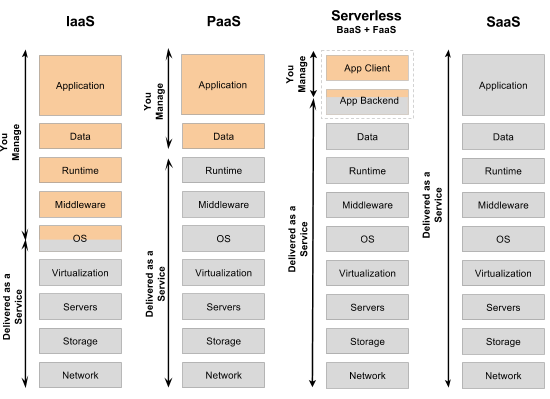
\includegraphics[width=\textwidth]{specify-io-cloud-comparison.png}
  \caption{Degree of automation when using serverless \parencite{wolf16serverless}}
  \label{fig:degreeOfAutomation}
\end{figure}

\begin{figure}[h]
  \centering
  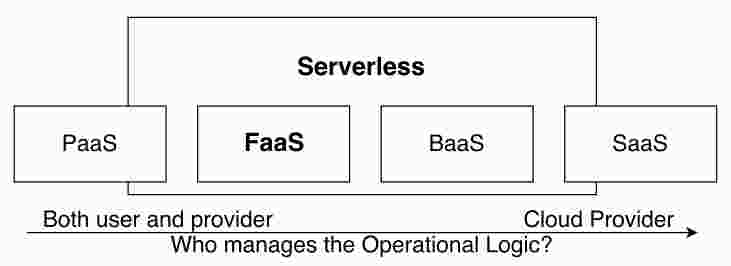
\includegraphics[width=\textwidth]{eyk17-cloud-comparison.jpg}
  \caption{Serverless and FaaS vs. PaaS and SaaS \parencite{van2017spec}}
  \label{fig:cloudSpectrum}
\end{figure}

Since the gap between PaaS and FaaS can be quite subtle it warrants further consideration. Indeed some sources, including \textcite{adzic2017serverless}, refer to FaaS as a new generation of PaaS offerings. Both models provide a high-level and elastic computing platform on which to implement custom business logic. There are however a number of substantial differences between the two models, which ultimately boil down to PaaS being an instance-based model (multiple server processes running on always-on server instances) as opposed to the on-demand resource allocation of FaaS -- or as \textcite{robert2016serverlessarchitectures} puts it, most PaaS applications are not geared towards bringing entire applications up and down for every request, whereas FaaS platforms do exactly this.

\textcite{albuquerque17faaspaas} derive a number of specific differences between PaaS and FaaS in their comparative analysis. First of all the units of deployment vary: in PaaS applications are deployed as services, compared to the more granular function-based deployment of FaaS. Second, PaaS instances are always running whereas serverless workloads are executed on-demand. Third, PaaS platforms, although supporting auto-scaling to some extent, require the developer to explicitly manage the scaling workflow and number of minimum instances. FaaS on the other hand scales transparently and on-demand without any need for resource pre-allocation. Perhaps most important distinction lies in billing: PaaS is billed by instantiated resources whether they're used or not, whereas FaaS is billed per-event on a millisecond granularity. The analysis concludes that PaaS is well suited for predictable or constant workloads with long or variable per-request execution times; FaaS in turn provides better cost benefit for unpredictable or seasonal workloads with short per-request execution times. It's also to be noted that PaaS doesn't suffer from limits on execution duration and many other restrictions of FaaS as described in section \ref{sec:limitations}.

Another recent cloud-native technology is Container-as-a-Service (CaaS)...
% compare to CaaS \parencite{cncf18serverlessWG}. Buyya17 describes containers. \textcite{robert2016serverlessarchitectures} also has a few words on the topic: scaling and Reduced packaging and deployment complexity

\section{Function-as-a-Service} \label{sec:faas}

Briefly describe the inner workings of a FaaS runtime. Describe the two supported execution models, synchronous and asynchronous, and how they relate to application design. The former is used to build a typical request-response flow, e.g. a REST API endpoint, whereas the latter relates to pub-sub and other event-driven flows. Give examples on the kind of triggers supported by serverless platforms (HTTP calls, messaging, database events, ...).

\textcite{fox17} present a useful short definition of serverless as a cloud-native platform for short-running, stateless computation and event-driven applications which scales up and down instantly and automatically and charges for actual usage at a millisecond granularity.

\textcite{spillner17snafu} presents the design and implementation of a research-friendly FaaS runtime. \textcite{mcgrath17implement} present the design of a novel performance-oriented serverless computing platform, discussing implementation challenges such as function scaling and container discovery, lifecycle, and reuse. \textcite{hendrickson16openlambda} present OpenLambda, an open-source platform for serverless computation, describing the key aspects of serverless computation and presenting numerous research challenges that must be addressed in the design and implementation of such systems.

\section{Use cases} \label{sec:useCases}

Introduce the main/intended use cases for serverless, as well as the more esoteric applications in literature.

\textcite{mcgrath16cloudEventParadigms} present two real-world applications utilizing cloud event architectures.

\textcite{malawski17executescientific} find that while serverless infrastructures are designed mainly for processing background tasks of Web and IoT applications, the simple mode of operation makes this approach easy to use and promising in scientific workflows too. \textcite{jonas17occupy} argue that a serverless execution model with stateless functions can enable radically-simpler, fundamentally elastic, and more user-friendly distributed data processing systems. \textcite{spillner18faaster} also find that in many domains of scientific and high-performance computing, solutions can be engineered based on simple functions which are executed on commercially offered or self-hosted FaaS platforms.

Introduce edge computing as a particularly strong driver for serverless. \textcite{glikson17devicelessedge} propose the novel paradigm of Deviceless Edge Computing that extends the serverless paradigm to the edge of the network, enabling IoT and Edge devices to be seamlessly integrated as application execution infrastructure. \textcite{nastic17analyticsedge} present a novel approach implementing cloud-supported, real-time data analytics in serverless edge-computing applications. \textcite{baresi17edgecomputing} propose a serverless architecture at the edge, bringing a highly scalable, intelligent and cost-effective use of edge infrastructure’s resources with minimal configuration and operation efforts.

\textcite{fouladi2017encoding} present a serverless video-processing framework. \textcite{yan16chatbot} present the architecture and prototype of a chatbot using a serverless platform, where developers compose stateless functions together to perform useful actions. \textcite{ishakian17neural} evaluate the suitability of a serverless computing environment for the inferencing of large neural network models. \textcite{ast17webcomponent} describe an approach of how to utilize serverless computing to enable self-contained web components by deploying Web Component business logic as cloud-hosted functions.

\section{Service providers} \label{sec:providers}

\textcite{lynn2017preliminary} provide an overview and multi-level feature analysis of seven enterprise serverless computing platforms. \textcite{baldini17currentTrends} also has a narrower survey of serverless platforms.

\textcite{malawski18benchmark} benchmark different cloud function providers.

\section{Security} \label{sec:security}

Address the security implications of serverless. Overall the consensus seems to be that compared to services maintaining their own servers and resources, serverless approach reduces the attack surface. However, research needs to understand the new security issues introduced by FaaS. For example, because the infrastructure can share resources among cloud-functions, what is the ideal security vs. performance/cost trade-off? \parencite{van2017spec}

\section{Economics of serverless} \label{sec:economics}

% Considering these differences, FaaS offers a more attractive economic proposition due to no danger of under- or overprovisioning of resources.
\textcite{eivy2017wary} and \textcite{villamizar2016infrastructure} both focus on the economic aspects of serverless. \textcite{adzic2017serverless} explain how novel design patterns are used to significantly optimize costs -- just running traditional web apps inside Lambda containers doesn't necessarily equate to savings. \textcite{adzic2017serverless} also report savings between 66 and 95\% in two case studies, and present a handly table comparing hosting prices for intermittent service tasks. \textcite{spillner17exploiting} exploits the control plane of AWS Lambda to implement services practically for free. \textcite{leitner16modelcost} present an approach to model deployment costs of AWS Lambda applications in real-time. \textcite{kuhlenkamp17costradamus} present another cost-tracing system that enables per-request cost-tracing for cloud-based software services, noting that cost testing should not only rely on isolated tests of single services but consider comprehensive end-to-end cost traces. \textcite{albuquerque17faaspaas} have a detailed price comparison running the same app in FaaS and PaaS.

\section{Drawbacks and limitations} \label{sec:limitations}

What to take into consideration when migrating to serverless?

\textcite{lloydserverless} analyze serverless performance and elasticity, identifying the cold start phenomenon. Differences in runtimes/languages, and larger library dependencies lead to slower starts. \textcite{oakes17pipsqueak} address the problem by caching package dependencies on platform-level.

\textcite{baldini17trilemma} identify three competing constraints in serverless function composition: functions should be considered as black boxes; function composition should obey a substitution principle with respect to synchronous invocation; and invocations should not be double-billed.

\textcite{robert2016serverlessarchitectures}, \textcite{adzic2017serverless} and \textcite{baldini17currentTrends} each list a number of limitations, including lack of strong SLA, vendor lock-in, short life-span, immature local development tools, statelessness and many others.

\textcite{kuhlenkamp17costradamus} discover two serverless cost tradeoffs: the retry cost effect and the cost ripple effect.

\textcite{malawski18benchmark} talk about interoperability challenges running a heterogeneous benchmark, as well as discussion on RAM allocation.

\textcite{cncf18serverlessWG} on technical immaturity, lack of interoperability, standardization, tools, documentation, best practices.

The need for circuit breakers (risk of DDoSing yourself) when interacting with non-serverless components like a database. Mention novel cloud-native database services like Google's Cloud Spanner and AWS Aurora. Figure out a source for this -- \textcite{hohpe2004enterprise} might have a relevant pattern.

Address maintainability: debugging serverless functions, following the flow of control can be tough.

Composing serverless functions is not like composing regular functions. All the difficulties of distributed computing -- message loss, timeouts and others -- apply and have to be handled. Possible solutions include retry policies, dead-letter queues and idempotent functions.

A full-fledged general-purpose serverless computing model is still a vision that needs to be achieved. \parencite{buyya2017manifesto}

Unlike the abstract concept of cloud functions, FaaS cannot completely abstract away all operation logic from the user. The FaaS user can still change parameters and configurations, such as the suggested memory size or number of CPUs of the underlying function host, which influence the operation of the deployed cloufunction. \parencite{van2017spec}

\chapter{Serverless design patterns}

Survey of serverless design patterns. \textcite{baldini17currentTrends} put the question as follows:

\begin{quote}
Will there be patterns for building serverless solutions? How do we combine low granularity basic building blocks of serverless into bigger solutions? How are we going to decompose apps into functions so that they optimize resource usage? For example how do we identify CPU-bound parts of applications built to run in serverless services? Can we use well-defined patterns for composing functions and external APIs? What should be done on the server vs. client (e.g., are thicker clients more appropriate here)? Are there lessons learned that can be applied from OOP design patterns, Enterprise Integration Patterns, etc.?
\end{quote}

\section{Serverless patterns}

% in the upcoming http://www.serverlessdesignpatterns.com/ book: primitive patterns (periodical cron job, messaging), API patterns (wrapper/proxy, facade, async), orchestration (one way chain, two way chain, fan out, fan in), pipes & filters (workflow and long running, streams), traditional (command, singleton). Traditional patterns hint to GoF, something to adopt from there?

A limited number of purely serverless design patters. \textcite{sbarski2017serverless} introduce five patterns -- Command, Messaging Priority queue, Fan-out and Pipes and filters -- but they seem mostly to be reinterpretations of classic Enterprise Integration Patterns.

Common low-level design patterns such as function chaining and fanout \href{https://github.com/yochay/serverlesspatterns}{in Github}.

\textcite{mcgrath16cloudEventParadigms} demonstrate a fan-out pattern, easily and performantly solving a large-scale image resizing task.

API Gateway and messaging patterns as described in platforms' own documentation. \parencite{awslambda0218}

\textcite{adzic2017serverless} suggest 3 methods for optimizing resource usage: use distributed authorization, let clients orchestrate workflows and allow clients to directly connect to AWS resources. The authors also discuss how paying only for actual utilization has two additional benefits of 1) removing incentives for bundling and 2) removing barriers to versioning: examples of serverless economics affecting architecture. Presenting these (or applications of these) as more formal patterns could be of some value.

\textcite{robert2016serverlessarchitectures} asks how big can FaaS functions get before they get unwieldy? Assuming we can atomically deploy a group of FaaS functions what are good ways of creating such groupings - do they map closely to how we’d currently clump logic into microservices or does the difference in architecture push us in a different direction? Extending this further what are good ways of creating hybrid architectures between FaaS and traditional ‘always on’ persistent server components?

Extending this further what are good ways of creating hybrid architect

\textcite{ast17webcomponent} describe self-contained web components with serverless backends.

\section{Enterprise Integration Patterns}

\textcite{hohpe2004enterprise} present a number of asynchronous messaging architectures in the seminal book on EIP. While predating the whole serverless phenomenon the patterns are still relevant. Hohpe even demonstrated implementing one of his patterns on top of Google's serverless platform \href{http://www.enterpriseintegrationpatterns.com/ramblings/google_cloud_functions.html}{in a blog post}.

\section{FaaSification}

\textcite{spillner17transformpython} describes an automated approach to transform monolithic Python code into modular FaaS units by partially automated decomposition. Doesn't really seem suitable for the web application migration process covered in this thesis but worth mentioning.

\chapter{Migration process}

Implement a subset of the target app in a serverless style, utilizing the surveyed patterns and keeping log of the tricky parts. In case the patterns prove unsuitable for the given problem, try to come up with an alternative solution.

Describe the web application to migrate.

Decide on the parts to migrate. Should demonstrate the features and limitations of serverless as outlined above. Possible features include
\begin{itemize}
  \item A simple REST API endpoint to showcase API Gateway and synchronous invocation. Shouldn't require any big changes to application code.
  \item Interaction between multiple services to demonstrate distributed transactions.
  \item A scheduled (cron) event.
  \item Interacting with an external SaaS service like Twilio, Auth0. Demonstrate event-driven invocation.
  \item others?
\end{itemize}

\chapter{Evaluation}

Evaluation the outcome of migration process. Estimate the effects on performance and hosting costs. Weigh in on maintainability, testability, developer experience etc.

\chapter{Conclusion}

What can we conclude about the research questions? Mention limitations and further research directions.

\printbibliography

\end{document}
